% ==============================================================================
% SCIENTIFIC CONFERENCE POSTER: EQUATORIAL PLASMA BUBBLES DETECTION
% Dimensions: 90 cm x 120 cm (Portrait)
% Built with: tikzposter package for LaTeX
% Authors: Alberto I. C. Vieira, Cosme A. O. B. Figueiredo, Tiago M. U. Araújo
% Contact: albertoivo@gmail.com
% Affiliations: Universidade Federal da Paraíba (UFPB) & UFCG
% ==============================================================================

\documentclass[25pt, a0paper, portrait]{tikzposter}

% Physical geometry: exactly 90 cm x 120 cm with balanced margins
\geometry{paperwidth=90cm, paperheight=120cm, margin=1.6cm}

% Core Packages
\usepackage[utf8]{inputenc}
\usepackage[T1]{fontenc}
\usepackage{lmodern}
\usepackage{amsmath,amssymb,amsfonts}
\usepackage{booktabs}
\usepackage{array}
\usepackage{graphicx}
\usepackage{xcolor}
\usepackage{microtype}
\usepackage{tikz}
\usetikzlibrary{shapes.geometric,arrows.meta,positioning,calc,shadows,fit,backgrounds}

% ------------------------------------------------------------------------------
% COLOR PALETTE (Sober, authoritative Space Weather & Deep Learning theme)
% ------------------------------------------------------------------------------
\definecolor{NavyDark}{HTML}{071326}      % Deep space midnight navy (Title banner)
\definecolor{NavyPrimary}{HTML}{0F2B59}   % Primary royal navy (Block titles)
\definecolor{SlateNavy}{HTML}{1A365D}     % Accent navy
\definecolor{PosterBg}{HTML}{F1F5F9}      % Ultra clean light slate background
\definecolor{CardBg}{HTML}{FFFFFF}        % Crisp white block content cards
\definecolor{AccentAmber}{HTML}{D97706}   % Amber / Gold accent for metrics & subtitle
\definecolor{AccentCyan}{HTML}{0284C7}    % High-tech cyan for AI & data flow
\definecolor{AccentGreen}{HTML}{15803D}   % Emerald green for high performance
\definecolor{AccentRed}{HTML}{DC2626}     % Crimson for Space Weather hazards
\definecolor{TextDark}{HTML}{0F172A}      % Slate 900 for dark text readability
\definecolor{TextMuted}{HTML}{475569}     % Slate 600 for captions and subtitles
\definecolor{BorderGray}{HTML}{CBD5E1}    % Subtle card border
\definecolor{CardHighlight}{HTML}{F8FAFC} % Subtle card background tint

% Apply theme and styles
\usetheme{Simple}
\useblockstyle[roundedcorners=14, linewidth=2pt, titleinnersep=7mm, bodyinnersep=7mm]{Default}

% Color assignments for tikzposter
\colorlet{backgroundcolor}{PosterBg}
\colorlet{framecolor}{NavyDark}
\colorlet{titlebgcolor}{NavyDark}
\colorlet{titlefgcolor}{white}
\colorlet{blocktitlebgcolor}{NavyPrimary}
\colorlet{blocktitlefgcolor}{white}
\colorlet{blockbodybgcolor}{CardBg}
\colorlet{blockbodyfgcolor}{TextDark}
\colorlet{innerblocktitlebgcolor}{AccentCyan}
\colorlet{innerblocktitlefgcolor}{white}
\colorlet{innerblockbodybgcolor}{CardHighlight}
\colorlet{innerblockbodyfgcolor}{TextDark}

% ------------------------------------------------------------------------------
% CUSTOM MACROS & FORMATTING
% ------------------------------------------------------------------------------
\newcommand{\posteritem}[2]{\noindent\textbf{\color{NavyPrimary}\textbullet~#1:} #2\par\vspace{3pt}}
\newcommand{\alertitem}[2]{\noindent\textbf{\color{AccentRed}\textbullet~#1:} #2\par\vspace{2pt}}
\newcommand{\successitem}[2]{\noindent\textbf{\color{AccentGreen}\textbullet~#1:} #2\par\vspace{2pt}}

% Stat Card Macro
\newcommand{\metricbox}[4]{% #1=Value, #2=Label, #3=Subtext, #4=BorderColor
    \fcolorbox{#4}{white}{%
        \parbox{11.6cm}{%
            \centering\vspace{5pt}
            {\bfseries\fontsize{36}{40}\selectfont\color{#4} #1}\\[3pt]
            {\bfseries\fontsize{17}{21}\selectfont\color{NavyDark} #2}\\[2pt]
            {\fontsize{13}{16}\selectfont\color{TextMuted} #3}\vspace{5pt}
        }%
    }%
}

% ------------------------------------------------------------------------------
% CUSTOM FULL-WIDTH TITLE BANNER (Edge-to-edge flush design)
% ------------------------------------------------------------------------------
\definetitlestyle{ModernHeader}{
    width=\paperwidth, roundedcorners=0, linewidth=0pt, innersep=1.2cm,
    titletotopverticalspace=0mm, titletoblockverticalspace=14mm,
    titlegraphictotitledistance=10pt
}{
   \draw[draw=none, fill=NavyDark]%
   (\titleposleft-1cm,\titleposbottom) rectangle (\titleposright+1cm,\titlepostop+1cm);
   \draw[draw=none, fill=AccentAmber]%
   (\titleposleft-1cm,\titleposbottom) rectangle (\titleposright+1cm,\titleposbottom+4pt);
}
\usetitlestyle{ModernHeader}

\makeatletter
\renewcommand{\TP@maketitle}{
    \centering
    \begin{minipage}[c]{0.14\linewidth}
        \centering
        \IfFileExists{logos/logo_ufpb.png}{%
            \includegraphics[height=3.6cm,keepaspectratio]{logos/logo_ufpb.png}%
        }{%
            \fcolorbox{BorderGray}{white}{%
                \parbox{0.92\linewidth}{%
                    \centering\vspace{8pt}
                    {\bfseries\fontsize{32}{36}\selectfont\color{NavyPrimary} UFPB}\\[3pt]
                    {\color{TextMuted}\fontsize{13}{16}\selectfont Univ. Federal da Paraíba}\\[3pt]
                    {\color{AccentCyan}\bfseries\fontsize{13}{16}\selectfont EMBRACE / INPE}\vspace{8pt}
                }%
            }%
        }
    \end{minipage}%
    \hfill
    \begin{minipage}[c]{0.70\linewidth}
        \centering
        {\bfseries \fontsize{42}{50}\selectfont\color{white} Detecting Equatorial Plasma Bubbles with Machine Learning \par}
        \vspace*{0.3em}
        {\color{AccentAmber}\bfseries \fontsize{22}{27}\selectfont A Physics-Informed 2DPCA and Stacking Ensemble Architecture for Operational Space Weather Monitoring \par}
        \vspace*{0.4em}
        {\fontsize{21}{25}\selectfont\color{white} \textbf{Alberto I. C. Vieira}$^{1, \ast}$, \textbf{Cosme A. O. B. Figueiredo}$^{2}$, \textbf{Tiago M. U. Araújo}$^{1}$ \par}
        \vspace*{0.25em}
        {\color{white!90}\fontsize{16}{20}\selectfont $^{1}$Universidade Federal da Paraíba (UFPB), João Pessoa - PB, Brazil \quad $^{2}$Universidade Federal de Campina Grande (UFCG), Campina Grande - PB, Brazil \par}
        \vspace*{0.25em}
        {\color{white!75}\fontsize{14}{18}\selectfont $^{\ast}$Contact: \texttt{albertoivo@gmail.com} \quad $\vert$ \quad Observational Data: EMBRACE / INPE All-Sky Imager Network}
    \end{minipage}%
    \hfill
    \begin{minipage}[c]{0.14\linewidth}
        \centering
        \IfFileExists{logos/logo_ufcg.png}{%
            \includegraphics[height=3.6cm,keepaspectratio]{logos/logo_ufcg.png}%
        }{%
            \fcolorbox{BorderGray}{white}{%
                \parbox{0.92\linewidth}{%
                    \centering\vspace{8pt}
                    {\bfseries\fontsize{32}{36}\selectfont\color{NavyPrimary} UFCG}\\[3pt]
                    {\color{TextMuted}\fontsize{13}{16}\selectfont Univ. Federal de Campina Grande}\\[3pt]
                    {\color{AccentAmber}\bfseries\fontsize{13}{16}\selectfont AI \& Space Weather}\vspace{8pt}
                }%
            }%
        }
    \end{minipage}
}
\makeatother

\title{Detecting Equatorial Plasma Bubbles with Machine Learning}

% Turn off default tikzposter watermark logo in bottom corner
\tikzposterlatexaffectionproofoff

\begin{document}

\maketitle

% ==============================================================================
% POSTER BODY: BALANCED 3-COLUMN ARCHITECTURE
% ==============================================================================
\begin{columns}

    % ==========================================================================
    % COLUMN 1: INTRODUCTION & PIPELINE METHODOLOGY
    % ==========================================================================
    \column{0.33}

    % --------------------------------------------------------------------------
    % SECTION 1: OBJECTIVE
    % --------------------------------------------------------------------------
    \block{\textbf{1. Objective}}{
        This work presents a \textbf{physics-informed machine learning architecture} for automated detection of Equatorial Plasma Bubbles (EPBs) in All-Sky Imager (ASI) imagery from the \textbf{EMBRACE/INPE} observatory network. Rather than feeding raw optical frames into resource-heavy deep convolutional networks, the pipeline integrates domain-specific preprocessing (Gaussian background subtraction + CLAHE), \textbf{Two-Dimensional Principal Component Analysis} ($k=5$) for spatial feature extraction preserving 2D correlations, and a heterogeneous \textbf{Stacking Ensemble} classifier (SVC + XGBoost + Random Forest with Logistic meta-regression). Physical interpretability is validated via \textbf{SHAP} attribution maps, and operational stability is demonstrated on continuous nocturnal observational sequences, delivering a fast ($<5$~ms/image), interpretable, and GPU-free solution for real-time space weather monitoring.
    }

    % --------------------------------------------------------------------------
    % SECTION 2: INTRODUCTION & PHYSICAL CHALLENGE
    % --------------------------------------------------------------------------
    \block{\textbf{2. Introduction \& Physical Challenge}}{
        \textbf{Equatorial Plasma Bubbles (EPBs)} are large-scale plasma density depletions generated in the post-sunset equatorial ionospheric F-region. Driven by steep vertical density gradients following solar terminator passage, low-density plasma wells up into the denser topside ionosphere via the non-linear \textbf{Rayleigh-Taylor Instability (RTI)}, forming turbulent depleted channels that drift eastward.

        \vspace{0.3em}
        % Critical Space Weather Hazards Alert Box
        \begin{center}
        \fcolorbox{AccentRed!80}{AccentRed!5}{%
            \parbox{0.94\linewidth}{%
                \vspace{2pt}
                {\bfseries\color{AccentRed}\fontsize{17}{21}\selectfont Critical Space Weather Hazards:}\par\vspace{2pt}
                \alertitem{GNSS Degradation}{Causes severe amplitude and phase scintillation in trans-ionospheric radio signals (L-band), inducing loss of carrier lock, positioning errors, and cycle slips in GPS, Galileo, and GLONASS.}
                \alertitem{Satellite Telecom Disruptions}{Severely degrades satellite communications, commercial aviation links, and defense trans-equatorial HF radio channels.}
                \vspace{2pt}
            }%
        }
        \end{center}

        \vspace{0.3em}
        \textbf{The Observational Challenge in All-Sky Imagers (ASI):}
        Optical monitoring of the \textbf{OI 630.0~nm} airglow emission (altitude $\sim$250--300~km) is the gold standard for regional 2D mapping of EPBs. However, automated detection is hampered by extreme optical and environmental noise:
        
        \vspace{0.2em}
        \posteritem{Diffuse Background Variations}{Drastic variations from lunar illumination phases, twilight gradients, and large-scale airglow fluctuations distort intensities.}
        \posteritem{Environmental \& Sensor Noise}{Passing tropospheric clouds, haze, star fields, optical vignetting, and camera dome glares mimic or obscure plasma depletions.}
        \posteritem{Bottlenecks of Prior Deep Learning}{Manual inspection is labor-intensive and subjective. Heavy Deep Learning (CNNs) demands prohibitive GPU compute, tears 2D spatial context when flattening matrices, and overfits to stationary background stars or camera borders.}
    }

    % --------------------------------------------------------------------------
    % SECTION 3: PIPELINE METHODOLOGY: PREPROCESSING, 2DPCA & SMOTE
    % --------------------------------------------------------------------------
    \block{\textbf{3. Pipeline Methodology: Preprocessing, 2DPCA \& SMOTE}}{
        Rather than feeding uncurated optical frames into standard neural networks, we engineered a physics-informed pipeline to strip ambient noise while accentuating plasma structures:

        \vspace{0.3em}
        % Scaled TikZ Pipeline Flowchart
        \begin{center}
        \resizebox{0.98\linewidth}{!}{
            
\begin{tikzpicture}[
                node distance=0.6cm,
                stepbox/.style={rectangle, draw=NavyPrimary, fill=white, rounded corners=8pt, line width=1.8pt, minimum height=1.5cm, text width=5.2cm, align=center, font=\fontsize{14}{17}\selectfont, drop shadow={shadow xshift=2pt, shadow yshift=-2pt, opacity=0.15}},
                arrow/.style={-{Stealth[scale=1.1]}, line width=2.5pt, color=AccentCyan}
            ]
                \node[stepbox, draw=NavyDark, fill=NavyDark!6] (raw) {\textbf{Raw ASI Image}\\OI 630 nm (EMBRACE)};
                \node[stepbox, right=0.6cm of raw] (gauss) {\textbf{Gaussian Subtraction}\\$\sigma = 10$ Background Model};
                \node[stepbox, right=0.6cm of gauss] (clahe) {\textbf{CLAHE Equalization}\\Clip Limit $= 0.03$};
                \node[stepbox, right=0.6cm of clahe] (norm) {\textbf{Dynamic Normalization}\\Pixel Scale to $[0, 1]$};
                
                \draw[arrow] (raw) -- (gauss);
                \draw[arrow] (gauss) -- (clahe);
                \draw[arrow] (clahe) -- (norm);
            \end{tikzpicture}
        }
        \end{center}

        \vspace{0.2em}
        \posteritem{Gaussian Background Subtraction ($\sigma = 10$)}{A large 2D Gaussian kernel models low-frequency diffuse illumination (moonlight, airglow gradient). Subtracting it isolates high-contrast depletion structures.}
        \posteritem{CLAHE Enhancement (Clip Limit $= 0.03$)}{Contrast Limited Adaptive Histogram Equalization operates on localized tiles, sharpening narrow vertical depletion tears without amplifying high-frequency sensor noise.}
        \posteritem{Dynamic Normalization \& Scaling}{Min-max dynamic normalization maps calibrated intensity distributions into $[0, 1]$, neutralizing cross-station sensor gain variations.}
    }


    % ==========================================================================
    % COLUMN 2: 2DPCA, MODEL ARCHITECTURE & PERFORMANCE
    % ==========================================================================
    \column{0.34}

    % --------------------------------------------------------------------------
    % SECTION 4: DIMENSIONALITY REDUCTION (2DPCA) & SMOTE
    % --------------------------------------------------------------------------
    \block{\textbf{4. Feature Extraction (2DPCA) \& SMOTE}}{
        Standard PCA flattens $m \times n$ matrices into $mn$-dimensional 1D vectors, destroying spatial topology and requiring unwieldy $mn \times mn$ covariance matrices. 
        In contrast, \textbf{Two-Dimensional PCA (2DPCA)} evaluates the image covariance matrix $G \in \mathbb{R}^{n \times n}$ directly from image matrices $A_j$:
        \begin{equation*}
            G = \frac{1}{M} \sum_{j=1}^{M} (A_j - \bar{A})^T (A_j - \bar{A})
        \end{equation*}
        
        \vspace{0.15em}
        \begin{minipage}[t]{0.485\linewidth}
            \begin{tikzfigure}[Explained variance saturating at $k=5$]
                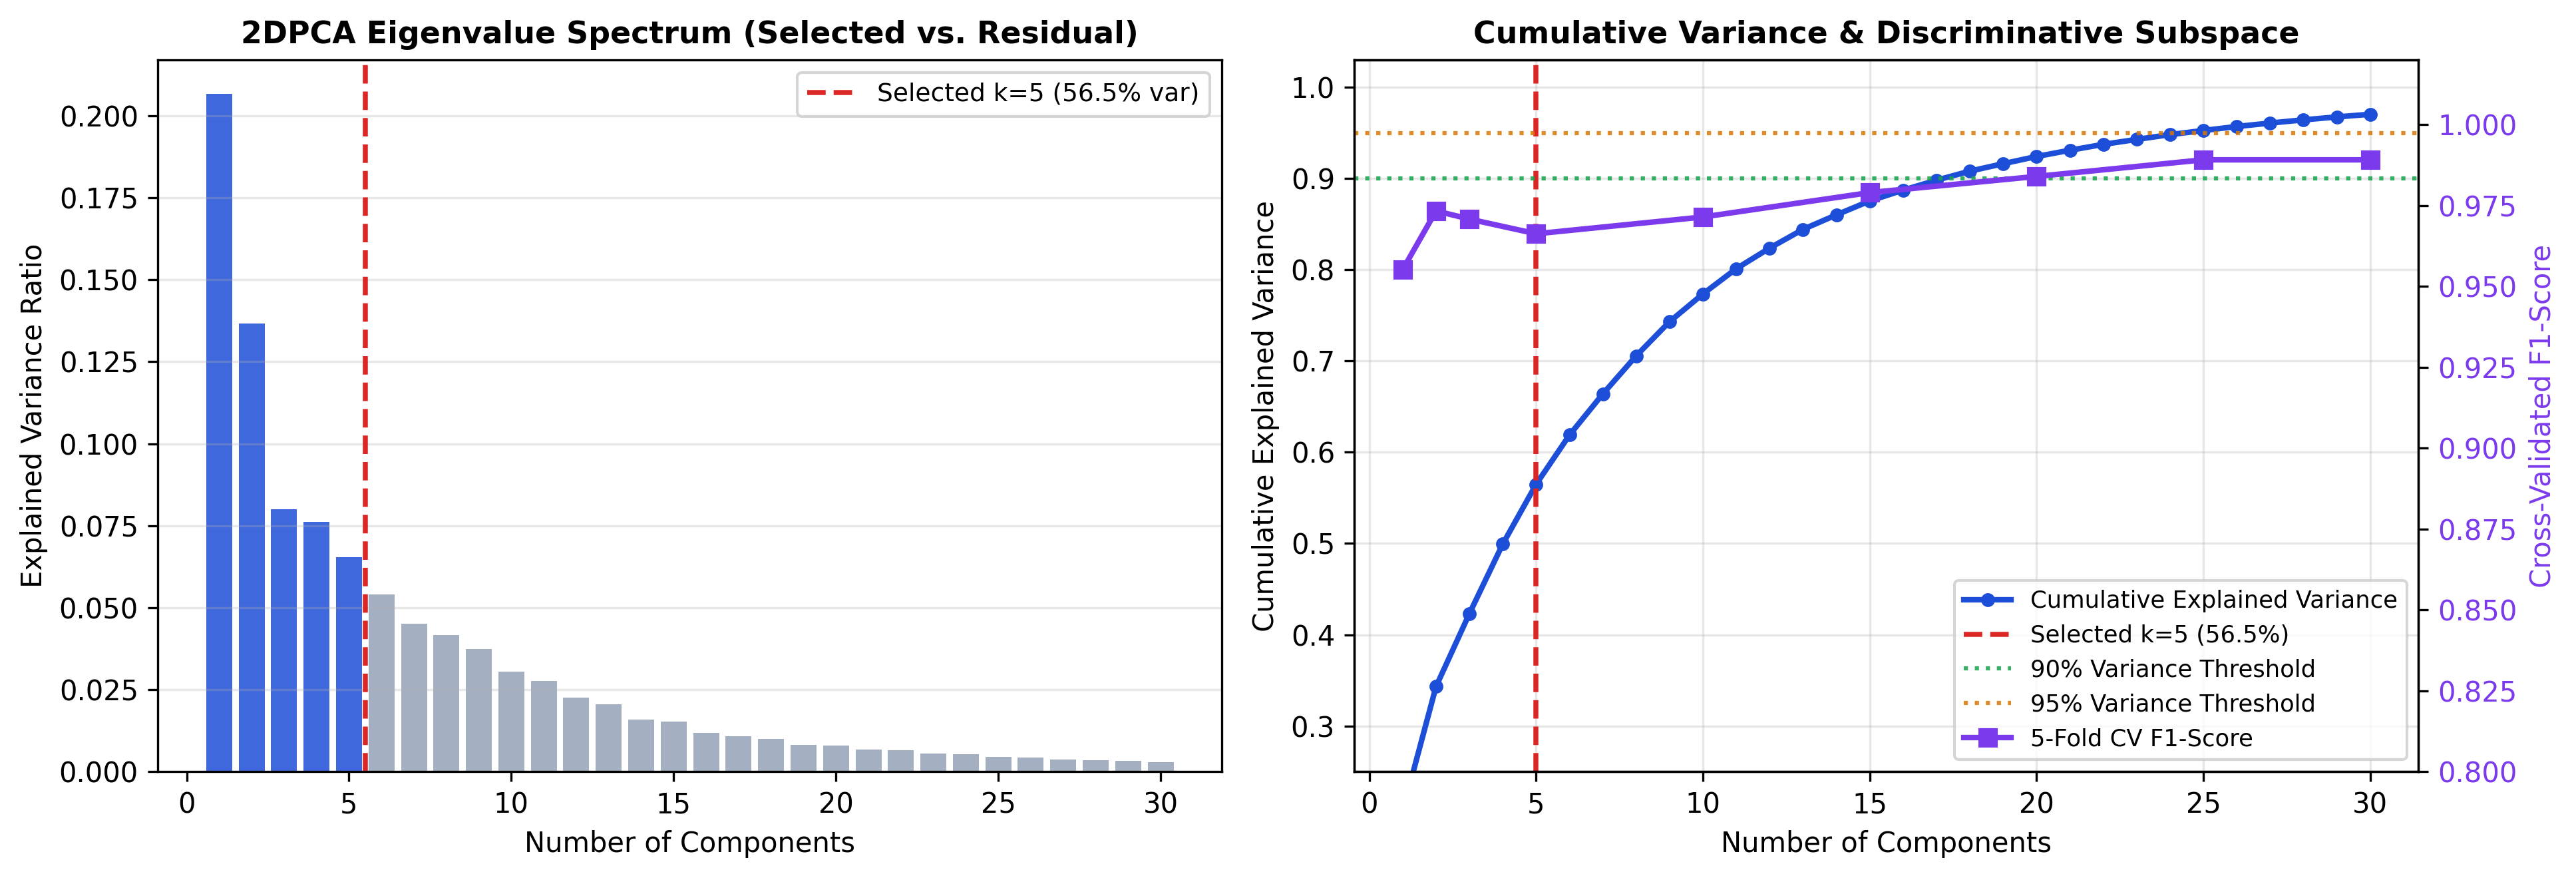
\includegraphics[width=0.98\linewidth,height=5.0cm,keepaspectratio]{figs/2dpca_variance.png}
            \end{tikzfigure}
        \end{minipage}%
        \hfill
        \begin{minipage}[t]{0.485\linewidth}
            \begin{tikzfigure}[2DPCA reconstruction of active EPB event]
                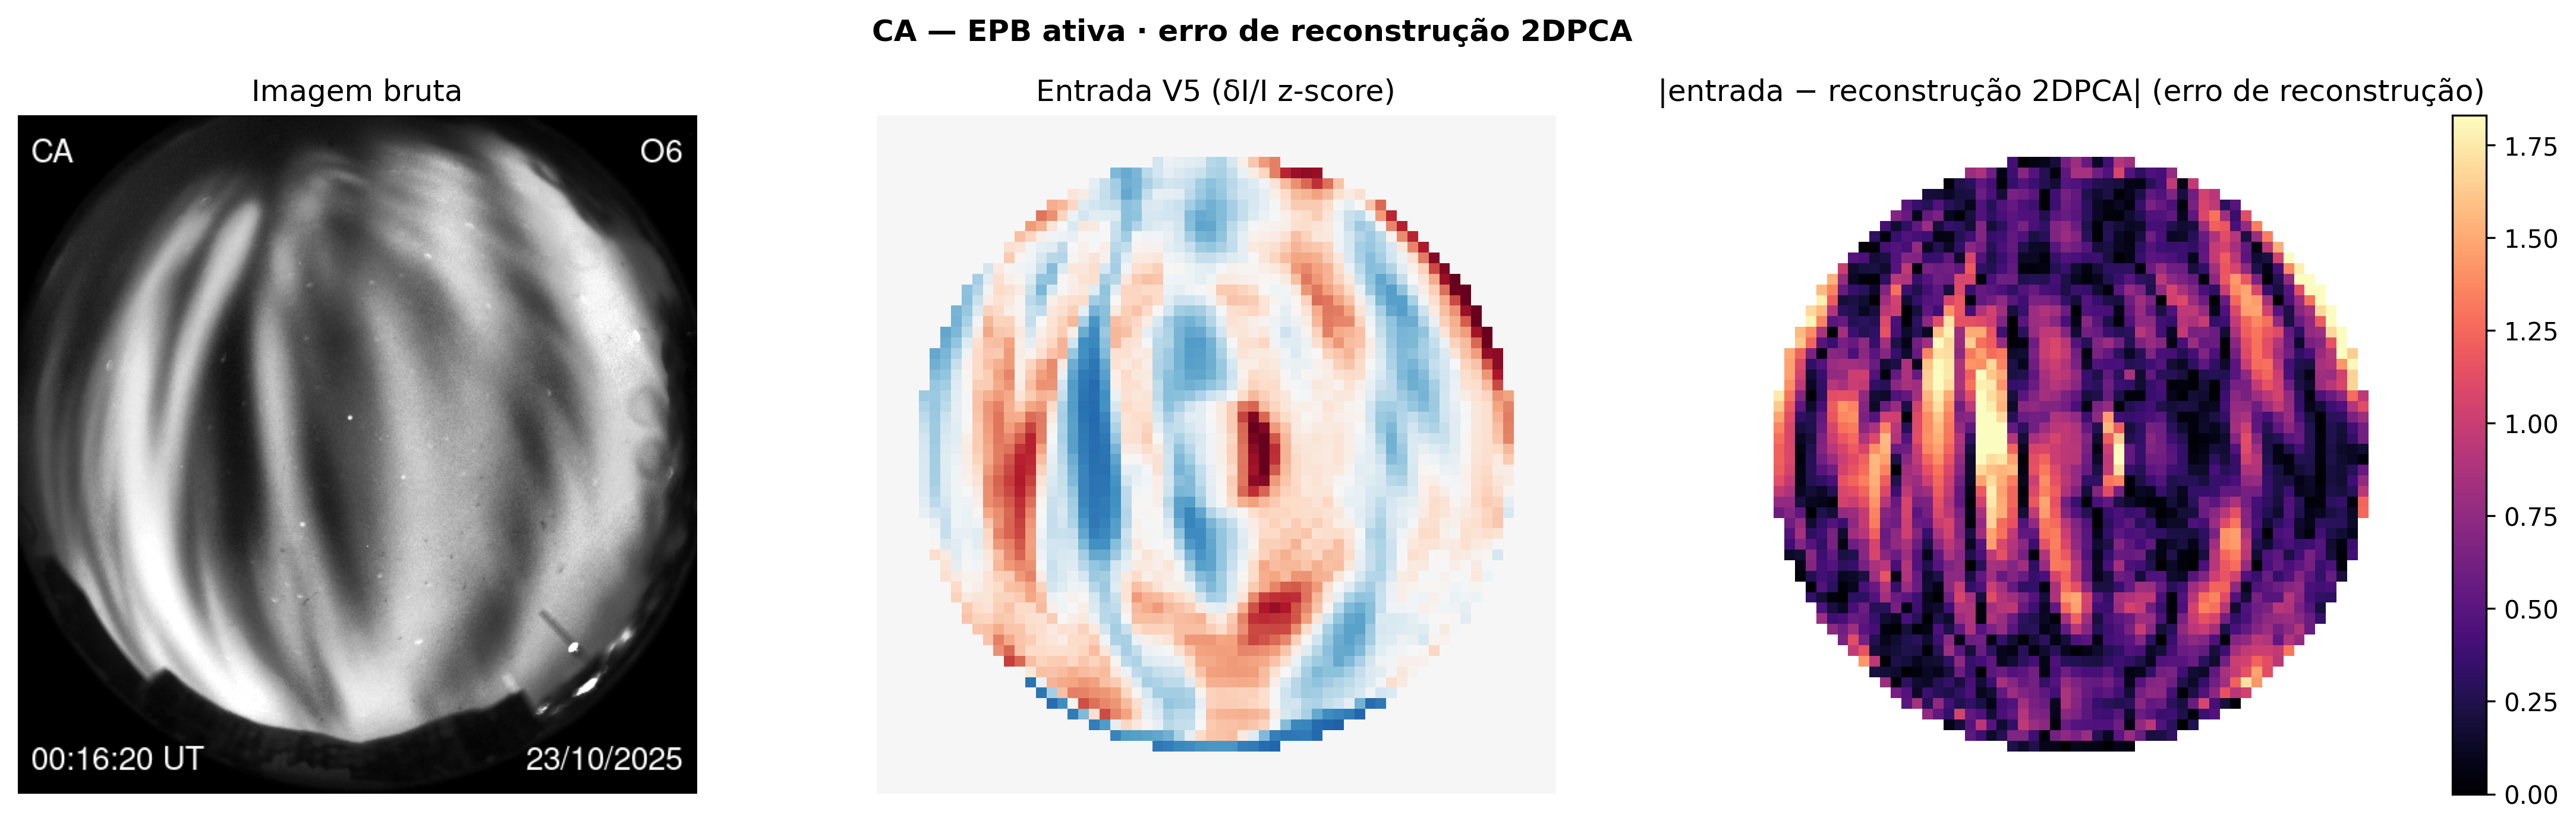
\includegraphics[width=0.98\linewidth,height=5.0cm,keepaspectratio]{figs/recon_error_with.png}
            \end{tikzfigure}
        \end{minipage}

        \vspace{0.15em}
        \posteritem{Optimal Subspace ($k = 5$)}{The first 5 principal components capture the structural morphology of EPBs, while higher components capture only random background noise.}
        \posteritem{Dual Class Balancing}{Controlled physical spatial augmentation combined with SMOTE directly in the 2DPCA feature space resolves severe operational class imbalance.}
    }

    % --------------------------------------------------------------------------
    % SECTION 5: MODEL ARCHITECTURE: STACKING ENSEMBLE
    % --------------------------------------------------------------------------
    \block{\textbf{5. Model Architecture: Stacking Ensemble}}{
        To maximize generalization and decision boundaries, we developed a heterogeneous \textbf{Stacking Ensemble} uniting three complementary machine learning paradigms:

        \vspace{0.25em}
        % TikZ Stacking Ensemble Architecture Diagram
        \begin{center}
        \resizebox{0.98\linewidth}{!}{
            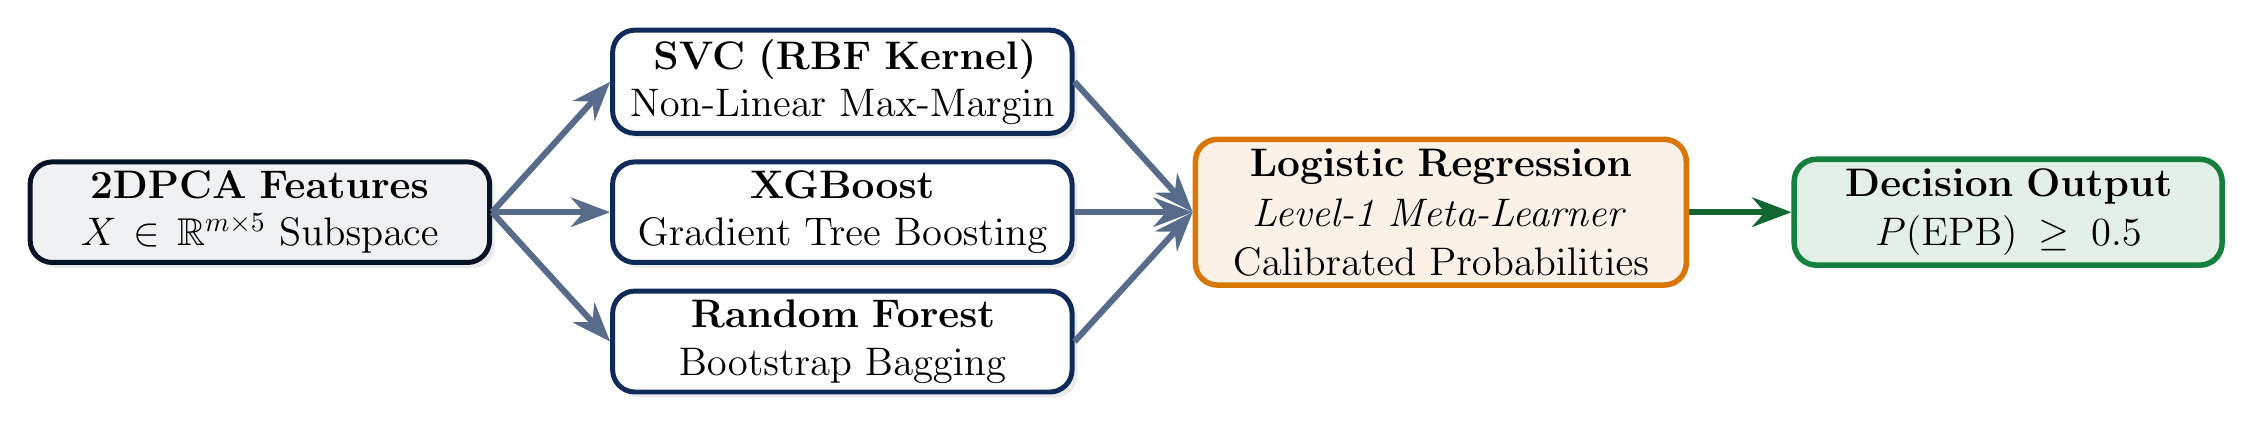
\begin{tikzpicture}[
                node distance=0.5cm,
                layerbox/.style={rectangle, draw=NavyPrimary, fill=white, rounded corners=8pt, line width=1.8pt, minimum height=1.15cm, text width=5.6cm, align=center, font=\fontsize{14}{17}\selectfont, drop shadow={shadow xshift=2pt, shadow yshift=-2pt, opacity=0.15}},
                metalayer/.style={rectangle, draw=AccentAmber, fill=AccentAmber!10, rounded corners=8pt, line width=2pt, minimum height=1.35cm, text width=6.0cm, align=center, font=\fontsize{15}{18}\selectfont},
                outputbox/.style={rectangle, draw=AccentGreen, fill=AccentGreen!12, rounded corners=8pt, line width=2pt, minimum height=1.15cm, text width=5.2cm, align=center, font=\fontsize{15}{18}\selectfont},
                flowarrow/.style={-{Stealth[scale=1.1]}, line width=2.2pt, color=NavyPrimary!70}
            ]
                \node[layerbox, draw=NavyDark, fill=NavyDark!6] (input) {\textbf{2DPCA Features}\\$X \in \mathbb{R}^{m \times 5}$ Subspace};
                
                \node[layerbox, right=1.5cm of input] (xgb) {\textbf{XGBoost}\\Gradient Tree Boosting};
                \node[layerbox, above=0.3cm of xgb] (svc) {\textbf{SVC (RBF Kernel)}\\Non-Linear Max-Margin};
                \node[layerbox, below=0.3cm of xgb] (rf) {\textbf{Random Forest}\\Bootstrap Bagging};
                
                \node[metalayer, right=1.5cm of xgb] (meta) {\textbf{Logistic Regression}\\\textit{Level-1 Meta-Learner}\\Calibrated Probabilities};
                \node[outputbox, right=1.3cm of meta] (out) {\textbf{Decision Output}\\$P(\text{EPB}) \ge 0.5$};
                
                % Arrows
                \draw[flowarrow] (input.east) -- (svc.west);
                \draw[flowarrow] (input.east) -- (xgb.west);
                \draw[flowarrow] (input.east) -- (rf.west);
                \draw[flowarrow] (svc.east) -- (meta.west);
                \draw[flowarrow] (xgb.east) -- (meta.west);
                \draw[flowarrow] (rf.east) -- (meta.west);
                \draw[flowarrow, color=AccentGreen!80!black] (meta.east) -- (out.west);
            \end{tikzpicture}
        }
        \end{center}

        \vspace{0.15em}
        \posteritem{Complementary Algorithmic Diversity}{SVC establishes maximum-margin hyperplanes; XGBoost captures complex non-linear feature splits; Random Forest prevents overfitting via bagging.}
        \posteritem{Meta-Learner Probability Blending}{The Logistic Regression meta-classifier optimally weights base learner predictions, guaranteeing smooth probabilistic calibration.}
    }

    % --------------------------------------------------------------------------
    % SECTION 6: OVERALL PERFORMANCE & THRESHOLD STABILITY
    % --------------------------------------------------------------------------
    \block{\textbf{6. Overall Performance \& Threshold Stability}}{
        Evaluation was conducted across \textbf{5-fold Cross-Validation} and confirmed on an independent observational test sequence ($N = 137$ nocturnal images):
        
        \vspace{0.25em}
        % 2x2 Metric Stat Dashboard Grid
        \begin{center}
        \begin{tabular}{@{}c@{\hspace{0.6cm}}c@{}}
            \metricbox{99.80\%}{Accuracy}{5-Fold Cross-Validation}{AccentGreen} &
            \metricbox{99.80\%}{F1-Score}{Harmonic Balance}{NavyPrimary} \\[5pt]
            \metricbox{100.0\%}{Sensitivity}{Zero Missed EPBs}{AccentAmber} &
            \metricbox{1.000}{ROC \& PR AUC}{Perfect Discrimination}{AccentCyan}
        \end{tabular}
        \end{center}

        \vspace{0.15em}
        \begin{tikzfigure}[Receiver Operating Characteristic (ROC), Precision-Recall (PR) curves, and Predicted Probabilities showing sharp separation at 0.5]
            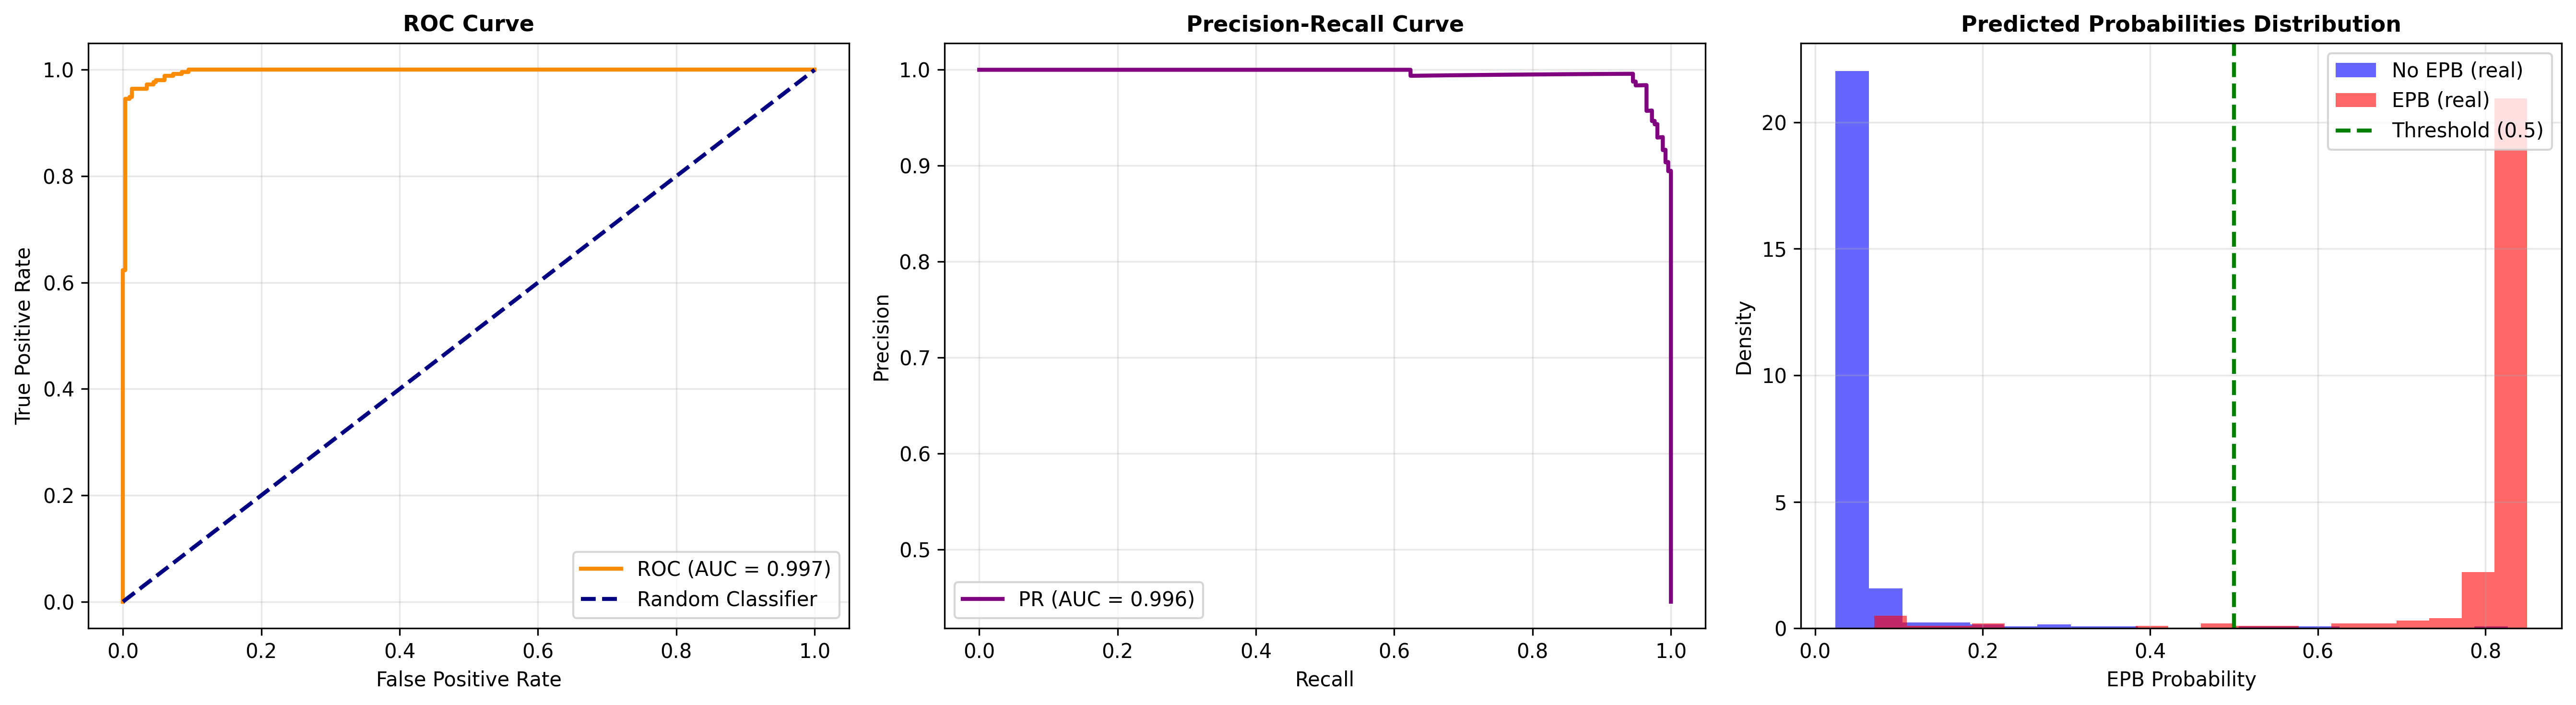
\includegraphics[width=0.98\linewidth,height=5.0cm,keepaspectratio]{figs/roc_pr_curves.png}
        \end{tikzfigure}

        \vspace{0.15em}
        \begin{minipage}[t]{0.485\linewidth}
            \begin{tikzfigure}[Confusion matrix ($N = 137$, 0 errors)]
                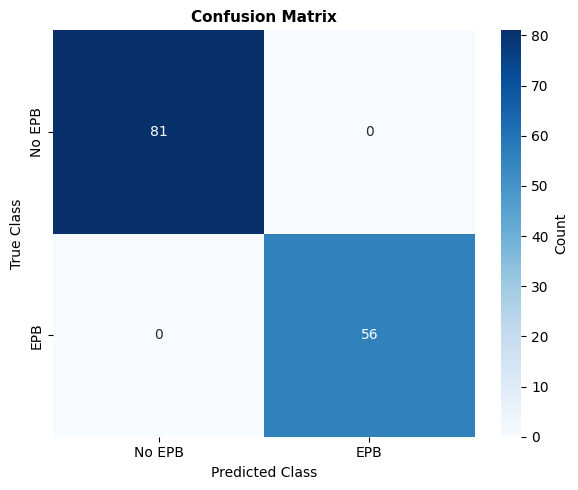
\includegraphics[width=0.98\linewidth,height=4.8cm,keepaspectratio]{figs/image_1.png}
            \end{tikzfigure}
        \end{minipage}%
        \hfill
        \begin{minipage}[t]{0.485\linewidth}
            \begin{tikzfigure}[{Threshold sensitivity ($t \in [0.1, 0.9]$)}]
                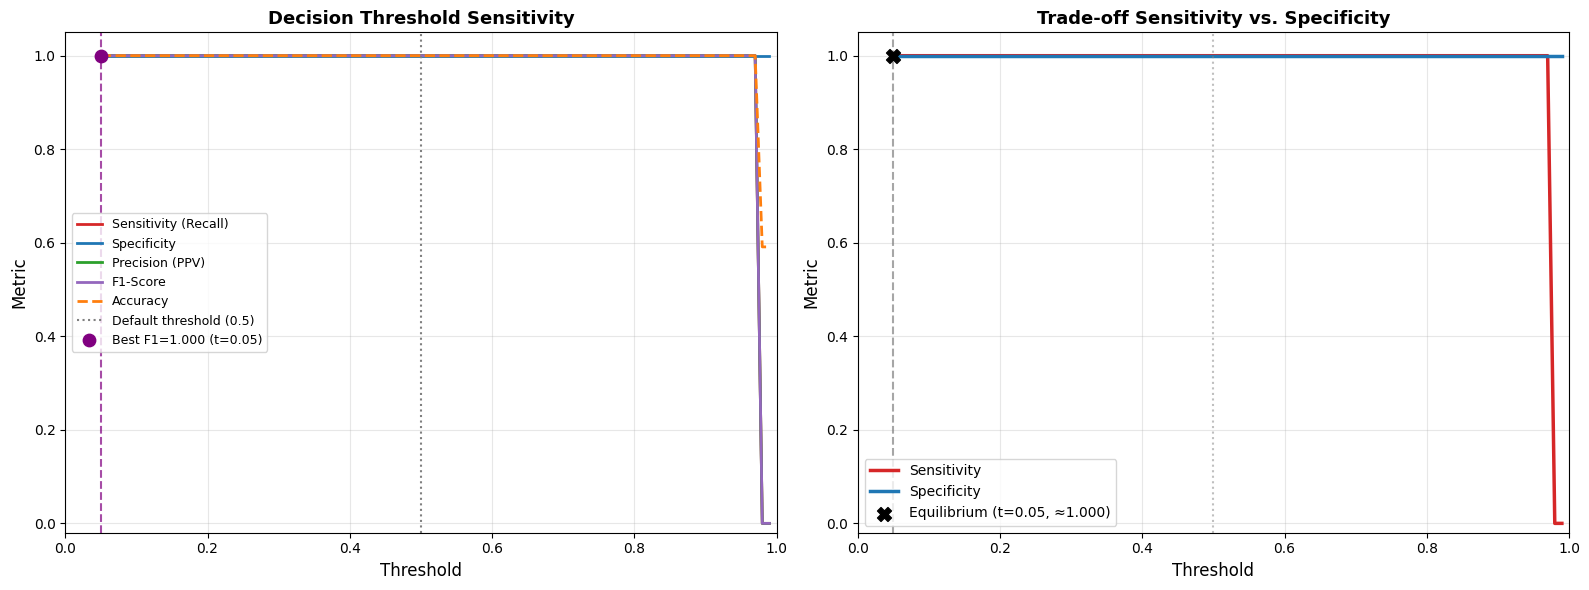
\includegraphics[width=0.98\linewidth,height=4.8cm,keepaspectratio]{figs/image_3.png}
            \end{tikzfigure}
        \end{minipage}

        \vspace{0.15em}
        \posteritem{Zero Test Errors ($N = 137$)}{81/81 True Negatives (100\%), 56/56 True Positives (100\%), 0 False Alarms (0.0\%), and 0 Missed EPBs (0.0\%).}
        \posteritem{Rock-Solid 0.5 Threshold Invariance}{Operational alert systems fail under brittle threshold tuning. Our Stacking Ensemble maintains constant performance across $t \in [0.10, 0.90]$, ensuring complete operational robustness.}
    }


    % ==========================================================================
    % COLUMN 3: VALIDATION, REAL-WORLD MONITORING & CONCLUSIONS
    % ==========================================================================
    \column{0.33}

    % --------------------------------------------------------------------------
    % SECTION 7: INTERPRETABILITY & GEOMAGNETIC ALIGNMENT (SHAP)
    % --------------------------------------------------------------------------
    \block{\textbf{7. Interpretability \& Physical Validation (SHAP)}}{
        Trust in AI space weather alerting requires physical verification. We integrated the \textbf{SHapley Additive exPlanations (SHAP)} framework to map pixel-level feature attributions:

        \vspace{0.25em}
        \begin{minipage}[t]{0.485\linewidth}
            \begin{tikzfigure}[Active EPB (Pred: 97.4\%): Field-aligned crests]
                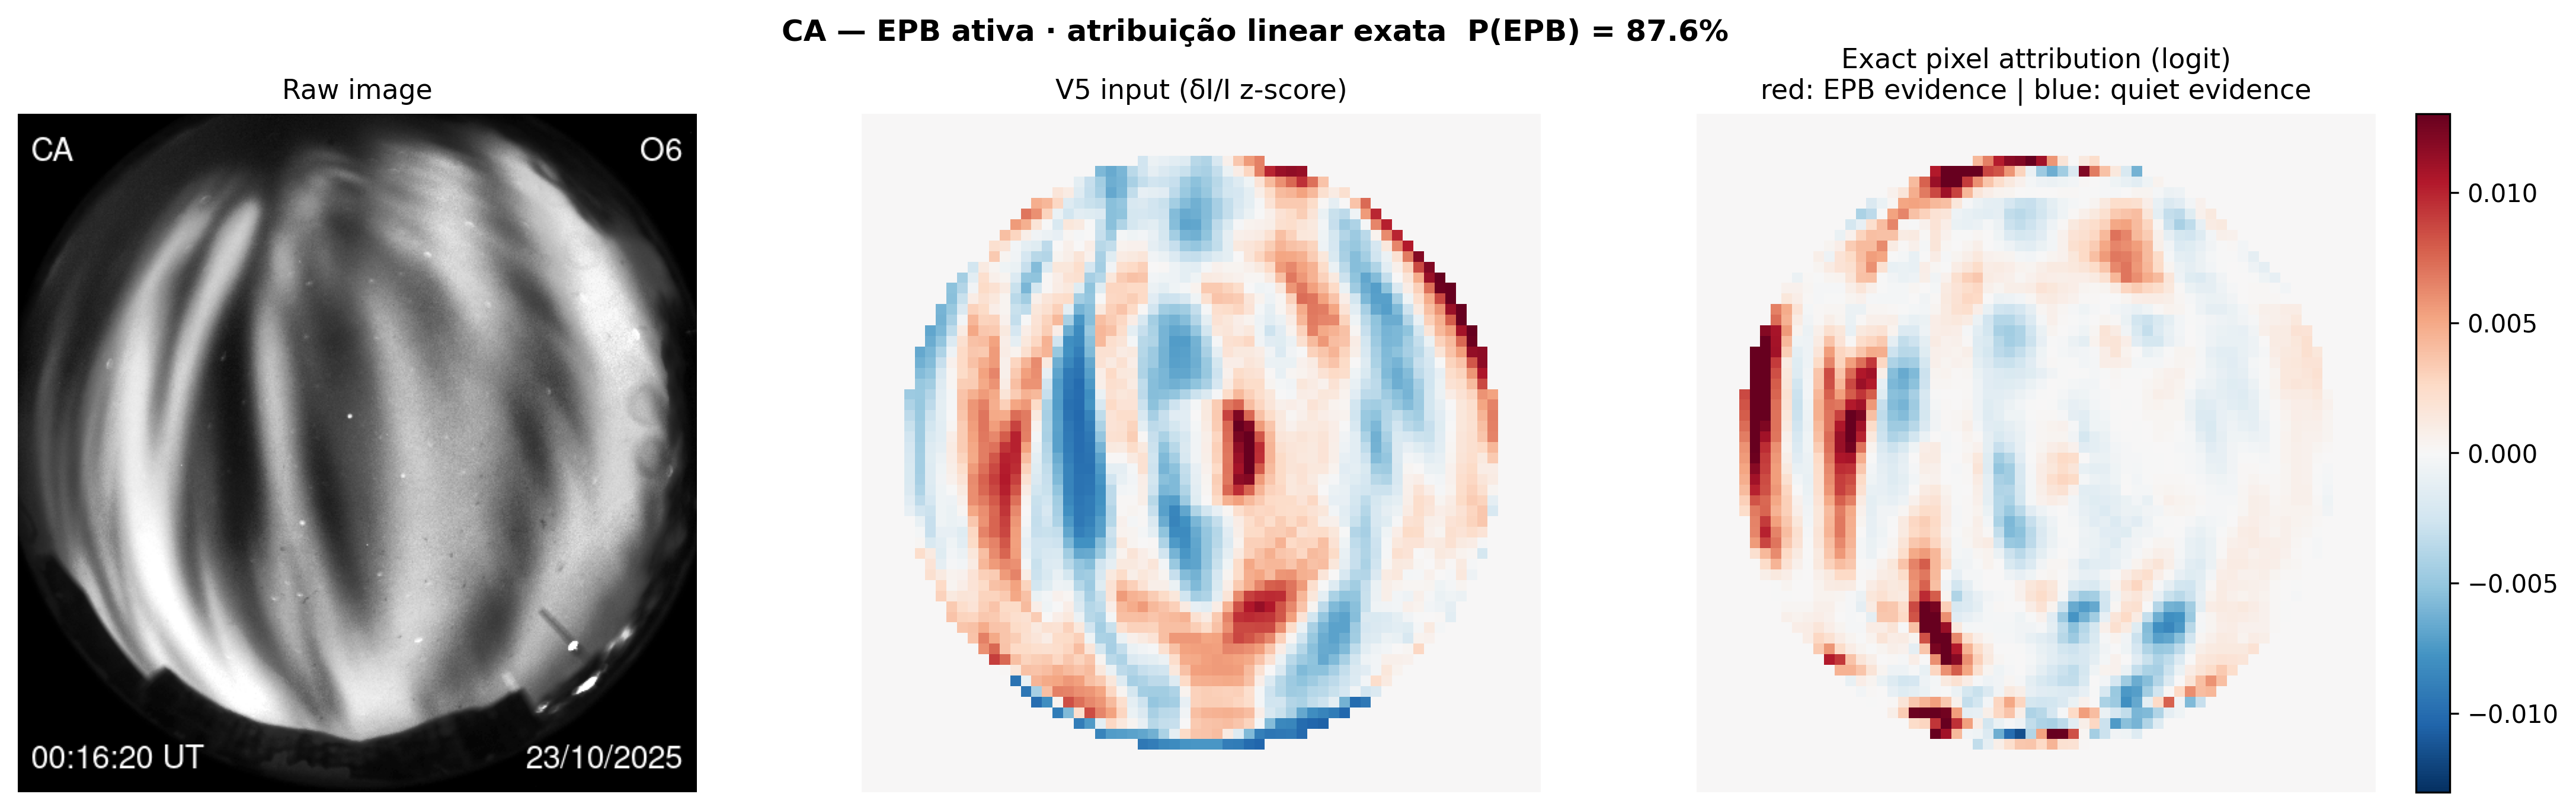
\includegraphics[width=0.98\linewidth,height=7.0cm,keepaspectratio]{figs/shap_analysis_with.png}
            \end{tikzfigure}
        \end{minipage}%
        \hfill
        \begin{minipage}[t]{0.485\linewidth}
            \begin{tikzfigure}[Quiet Night (Pred: 2.4\%): Diffuse background]
                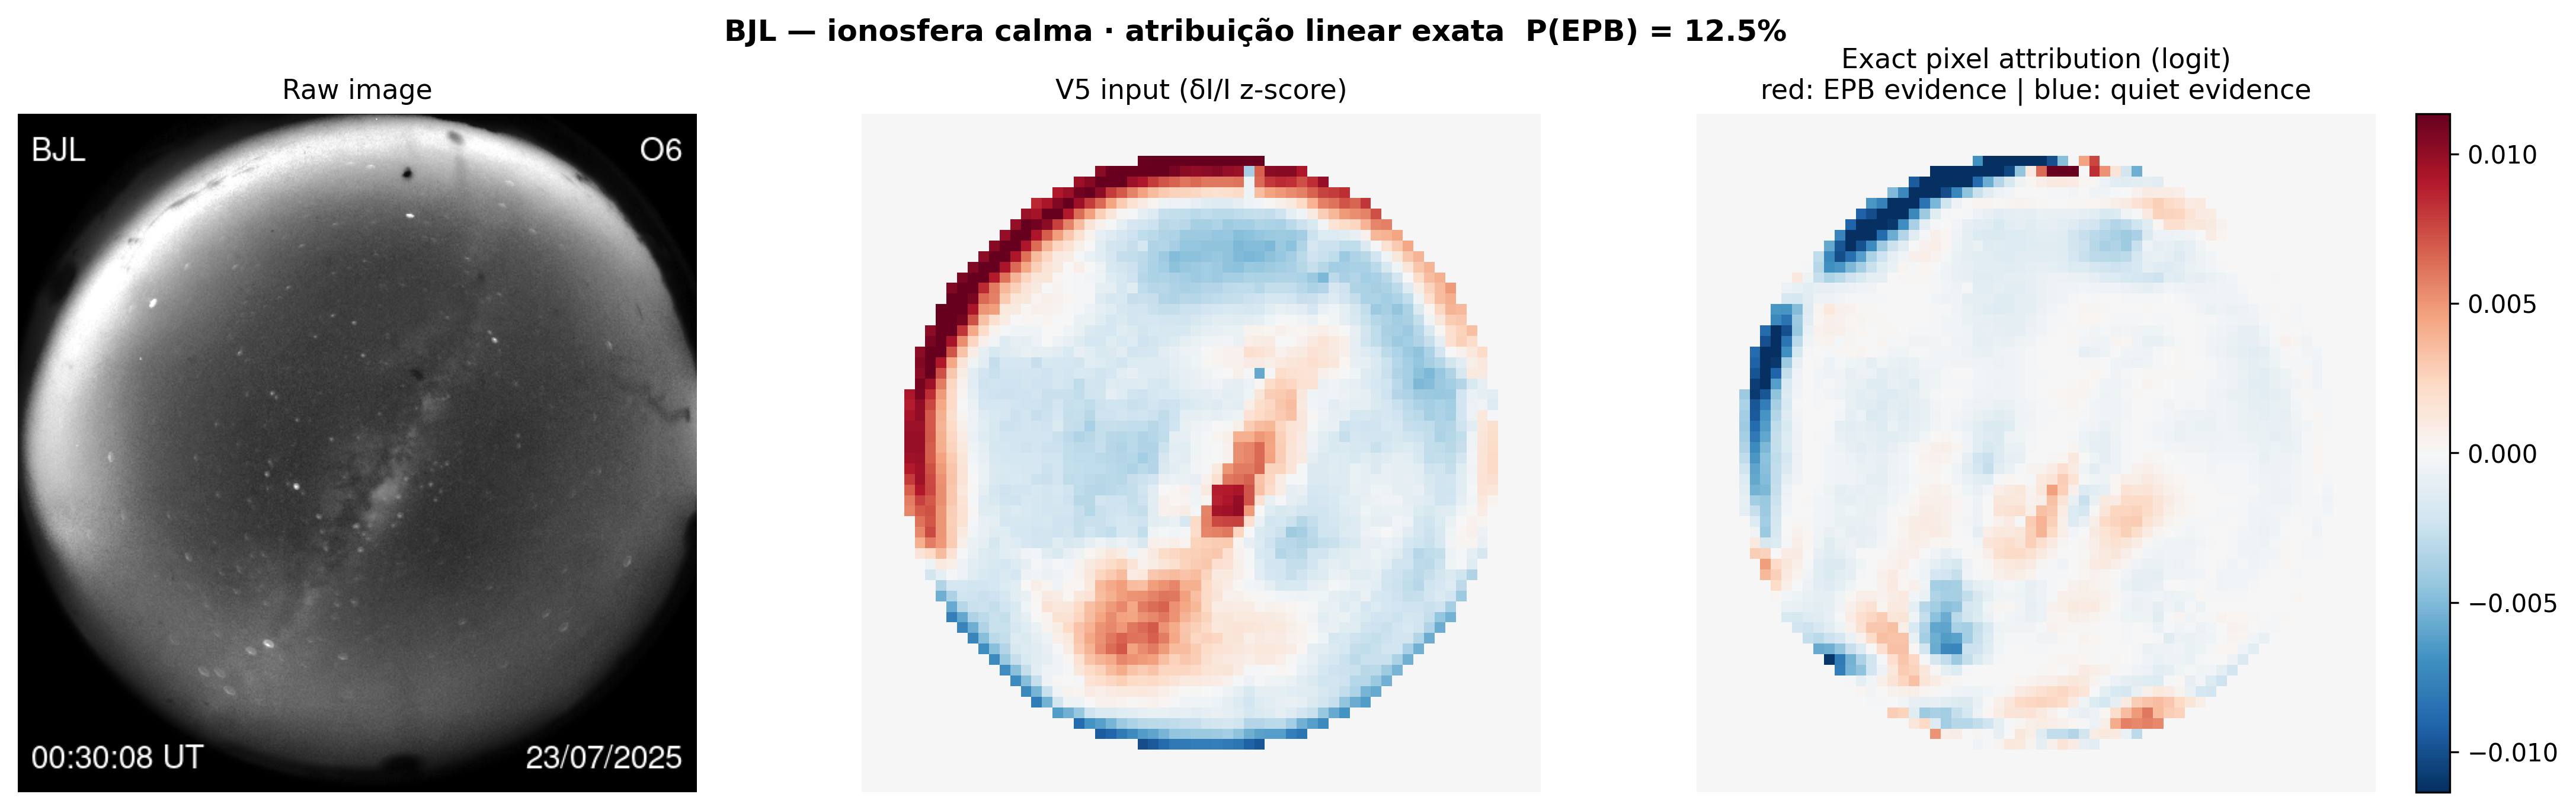
\includegraphics[width=0.98\linewidth,height=7.0cm,keepaspectratio]{figs/shap_analysis_without.png}
            \end{tikzfigure}
        \end{minipage}

        \vspace{0.25em}
        \posteritem{Compliance with Geomagnetic Field Lines}{Positive attributions (red) follow the vertically oriented plasma depletion bands rising into the upper field of view, strictly adhering to the north-south geomagnetic field line geometry in the Brazilian equatorial sector.}
        \posteritem{Artifact Immunity}{Background stars, city lighting, and camera dome borders receive zero or negative attribution, proving the model detects \textbf{true Rayleigh-Taylor dynamics} rather than camera noise.}
    }

    % --------------------------------------------------------------------------
    % SECTION 8: CONTINUOUS OPERATIONAL MONITORING (BJL & CA)
    % --------------------------------------------------------------------------
    \block{\textbf{8. Continuous Operational Monitoring (BJL \& CA)}}{
        The system was validated over continuous multi-hour nocturnal sequences from the EMBRACE / INPE observatory network:
        
        \vspace{0.25em}
        \begin{tikzfigure}[\textbf{Bom Jesus da Lapa (BJL)} Quiet Night (22--23 July 2025; 230 frames). Predicted probability remains at baseline (avg: 2.6\%; 0/230 EPBs)]
            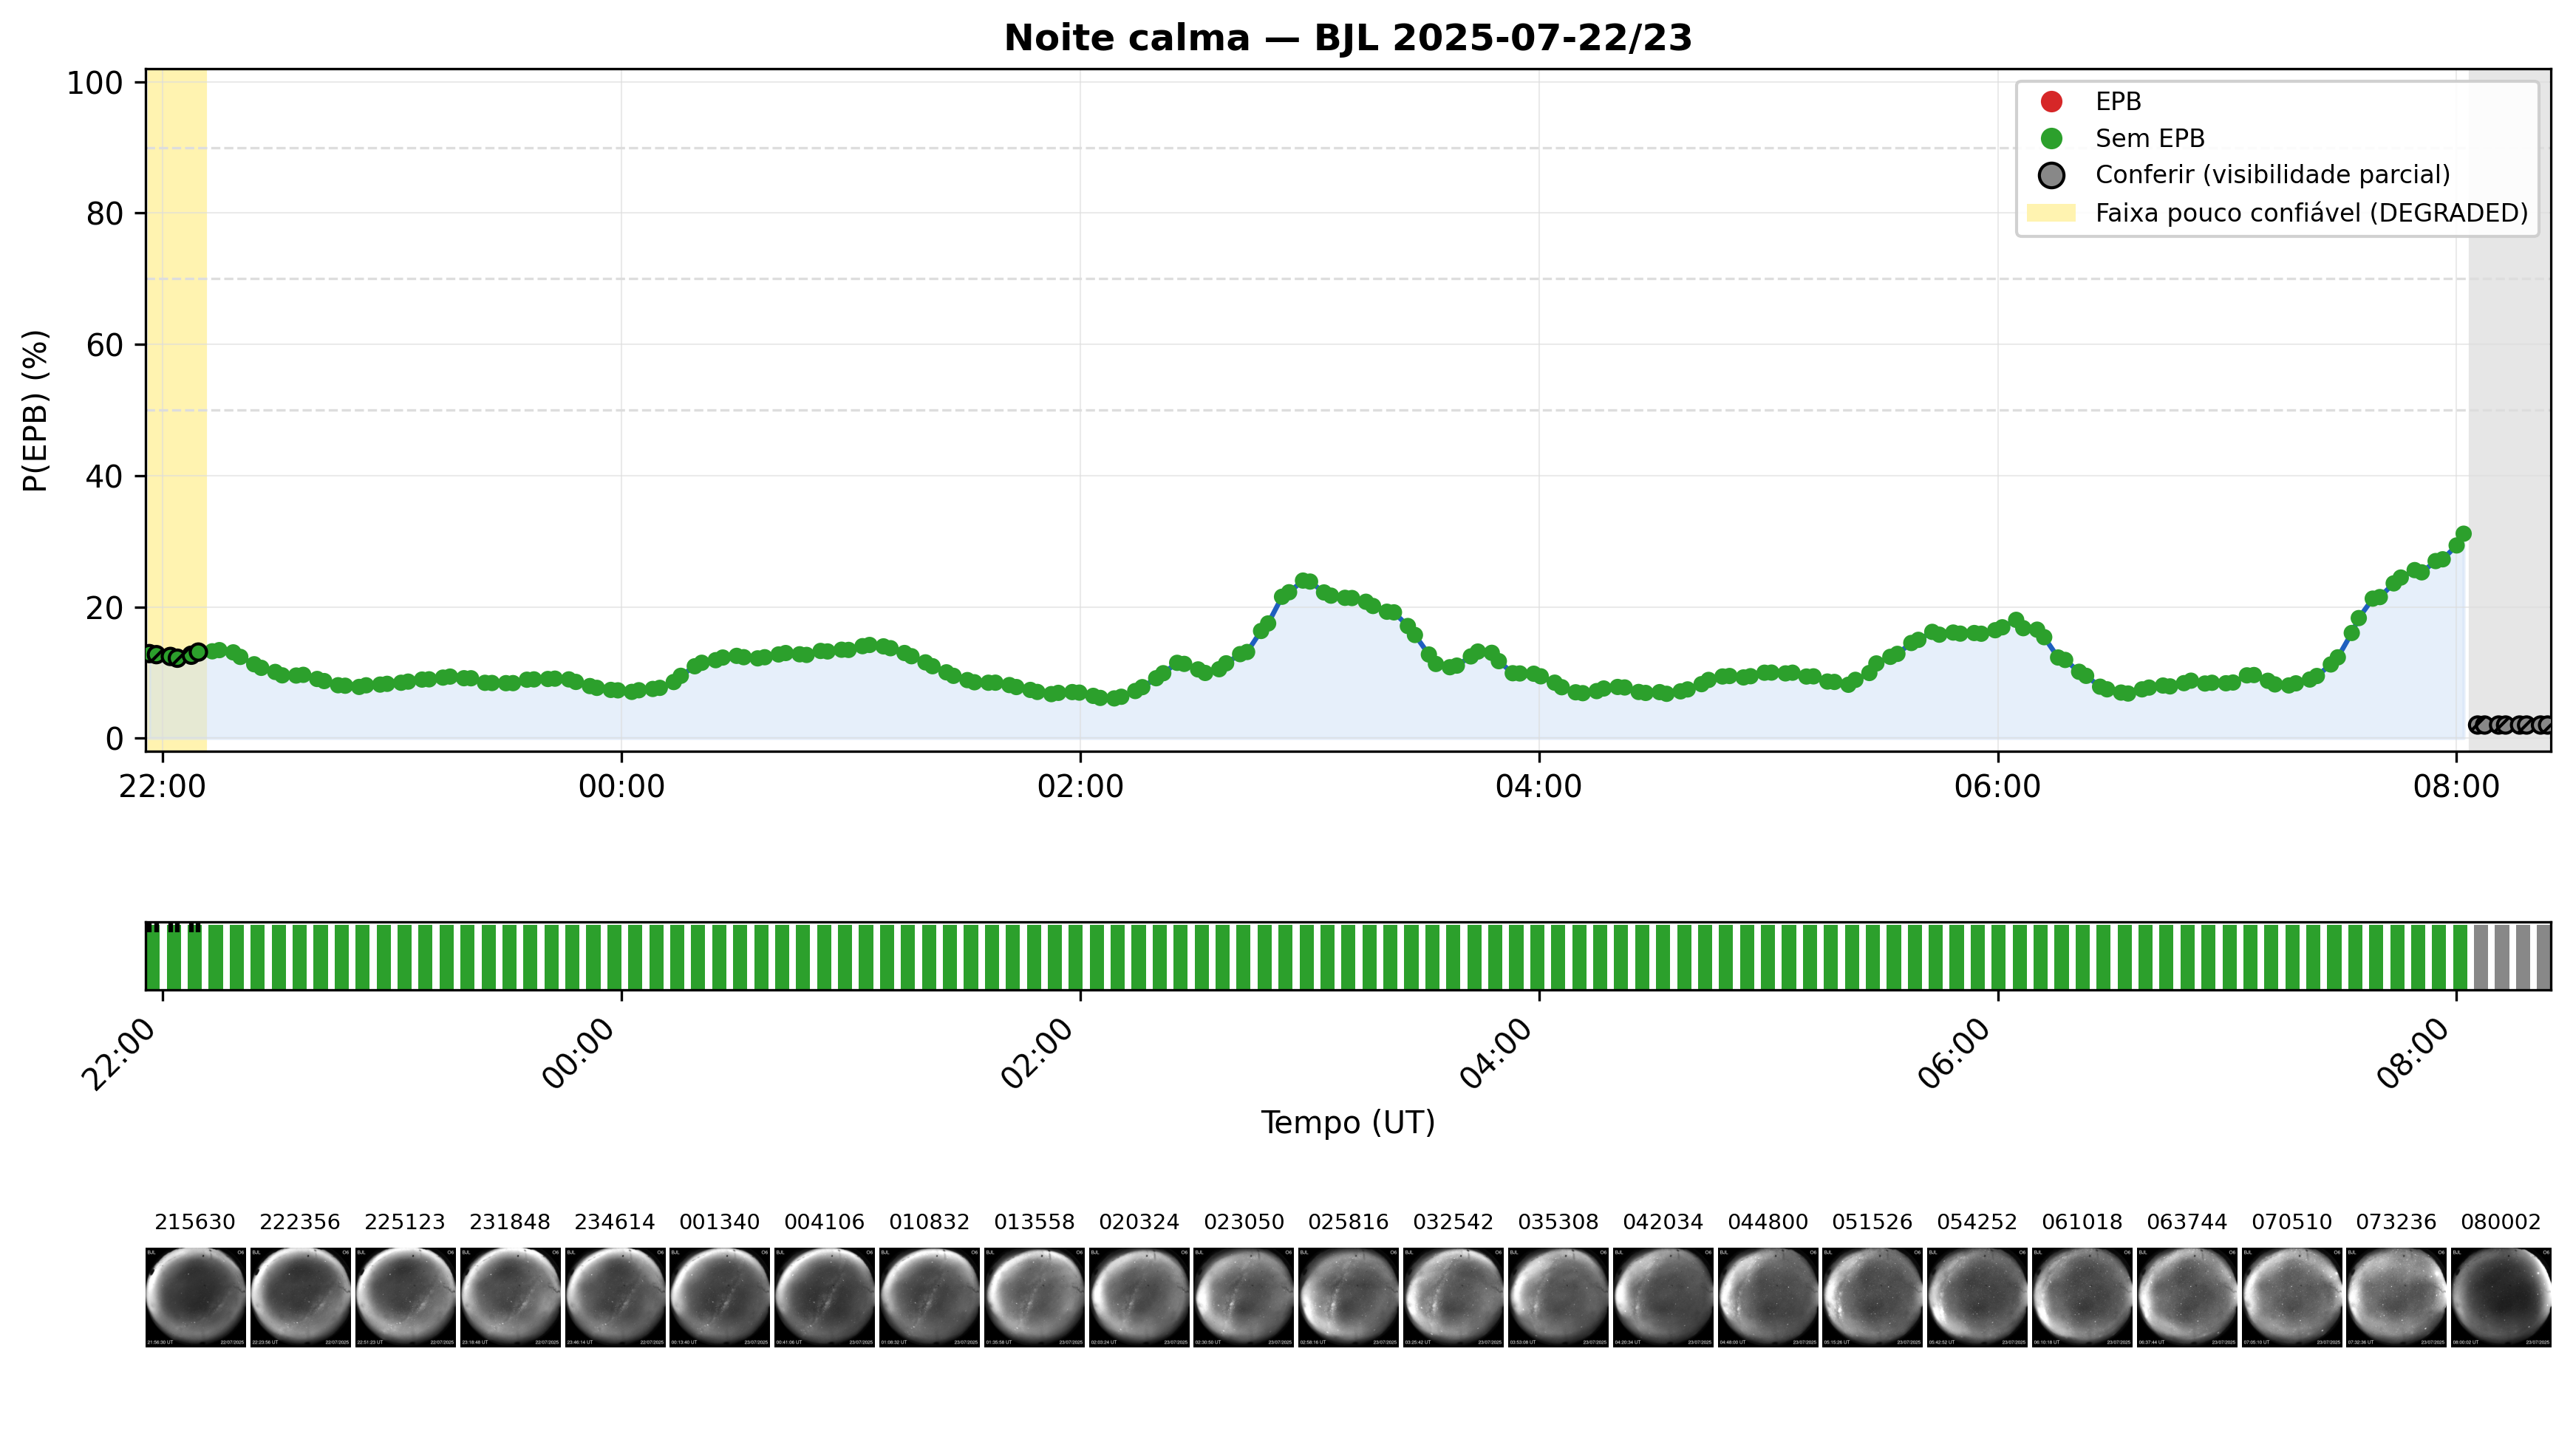
\includegraphics[width=0.98\linewidth,height=6.6cm,keepaspectratio]{figs/temporal_without_epb.png}
        \end{tikzfigure}

        \vspace{0.25em}
        \begin{tikzfigure}[\textbf{Cachoeira Paulista (CA)} Active Night (22--23 Oct 2025; 140 frames). Rapid onset detection and sustained tracking (avg: 91.5\%; 140/140 EPBs)]
            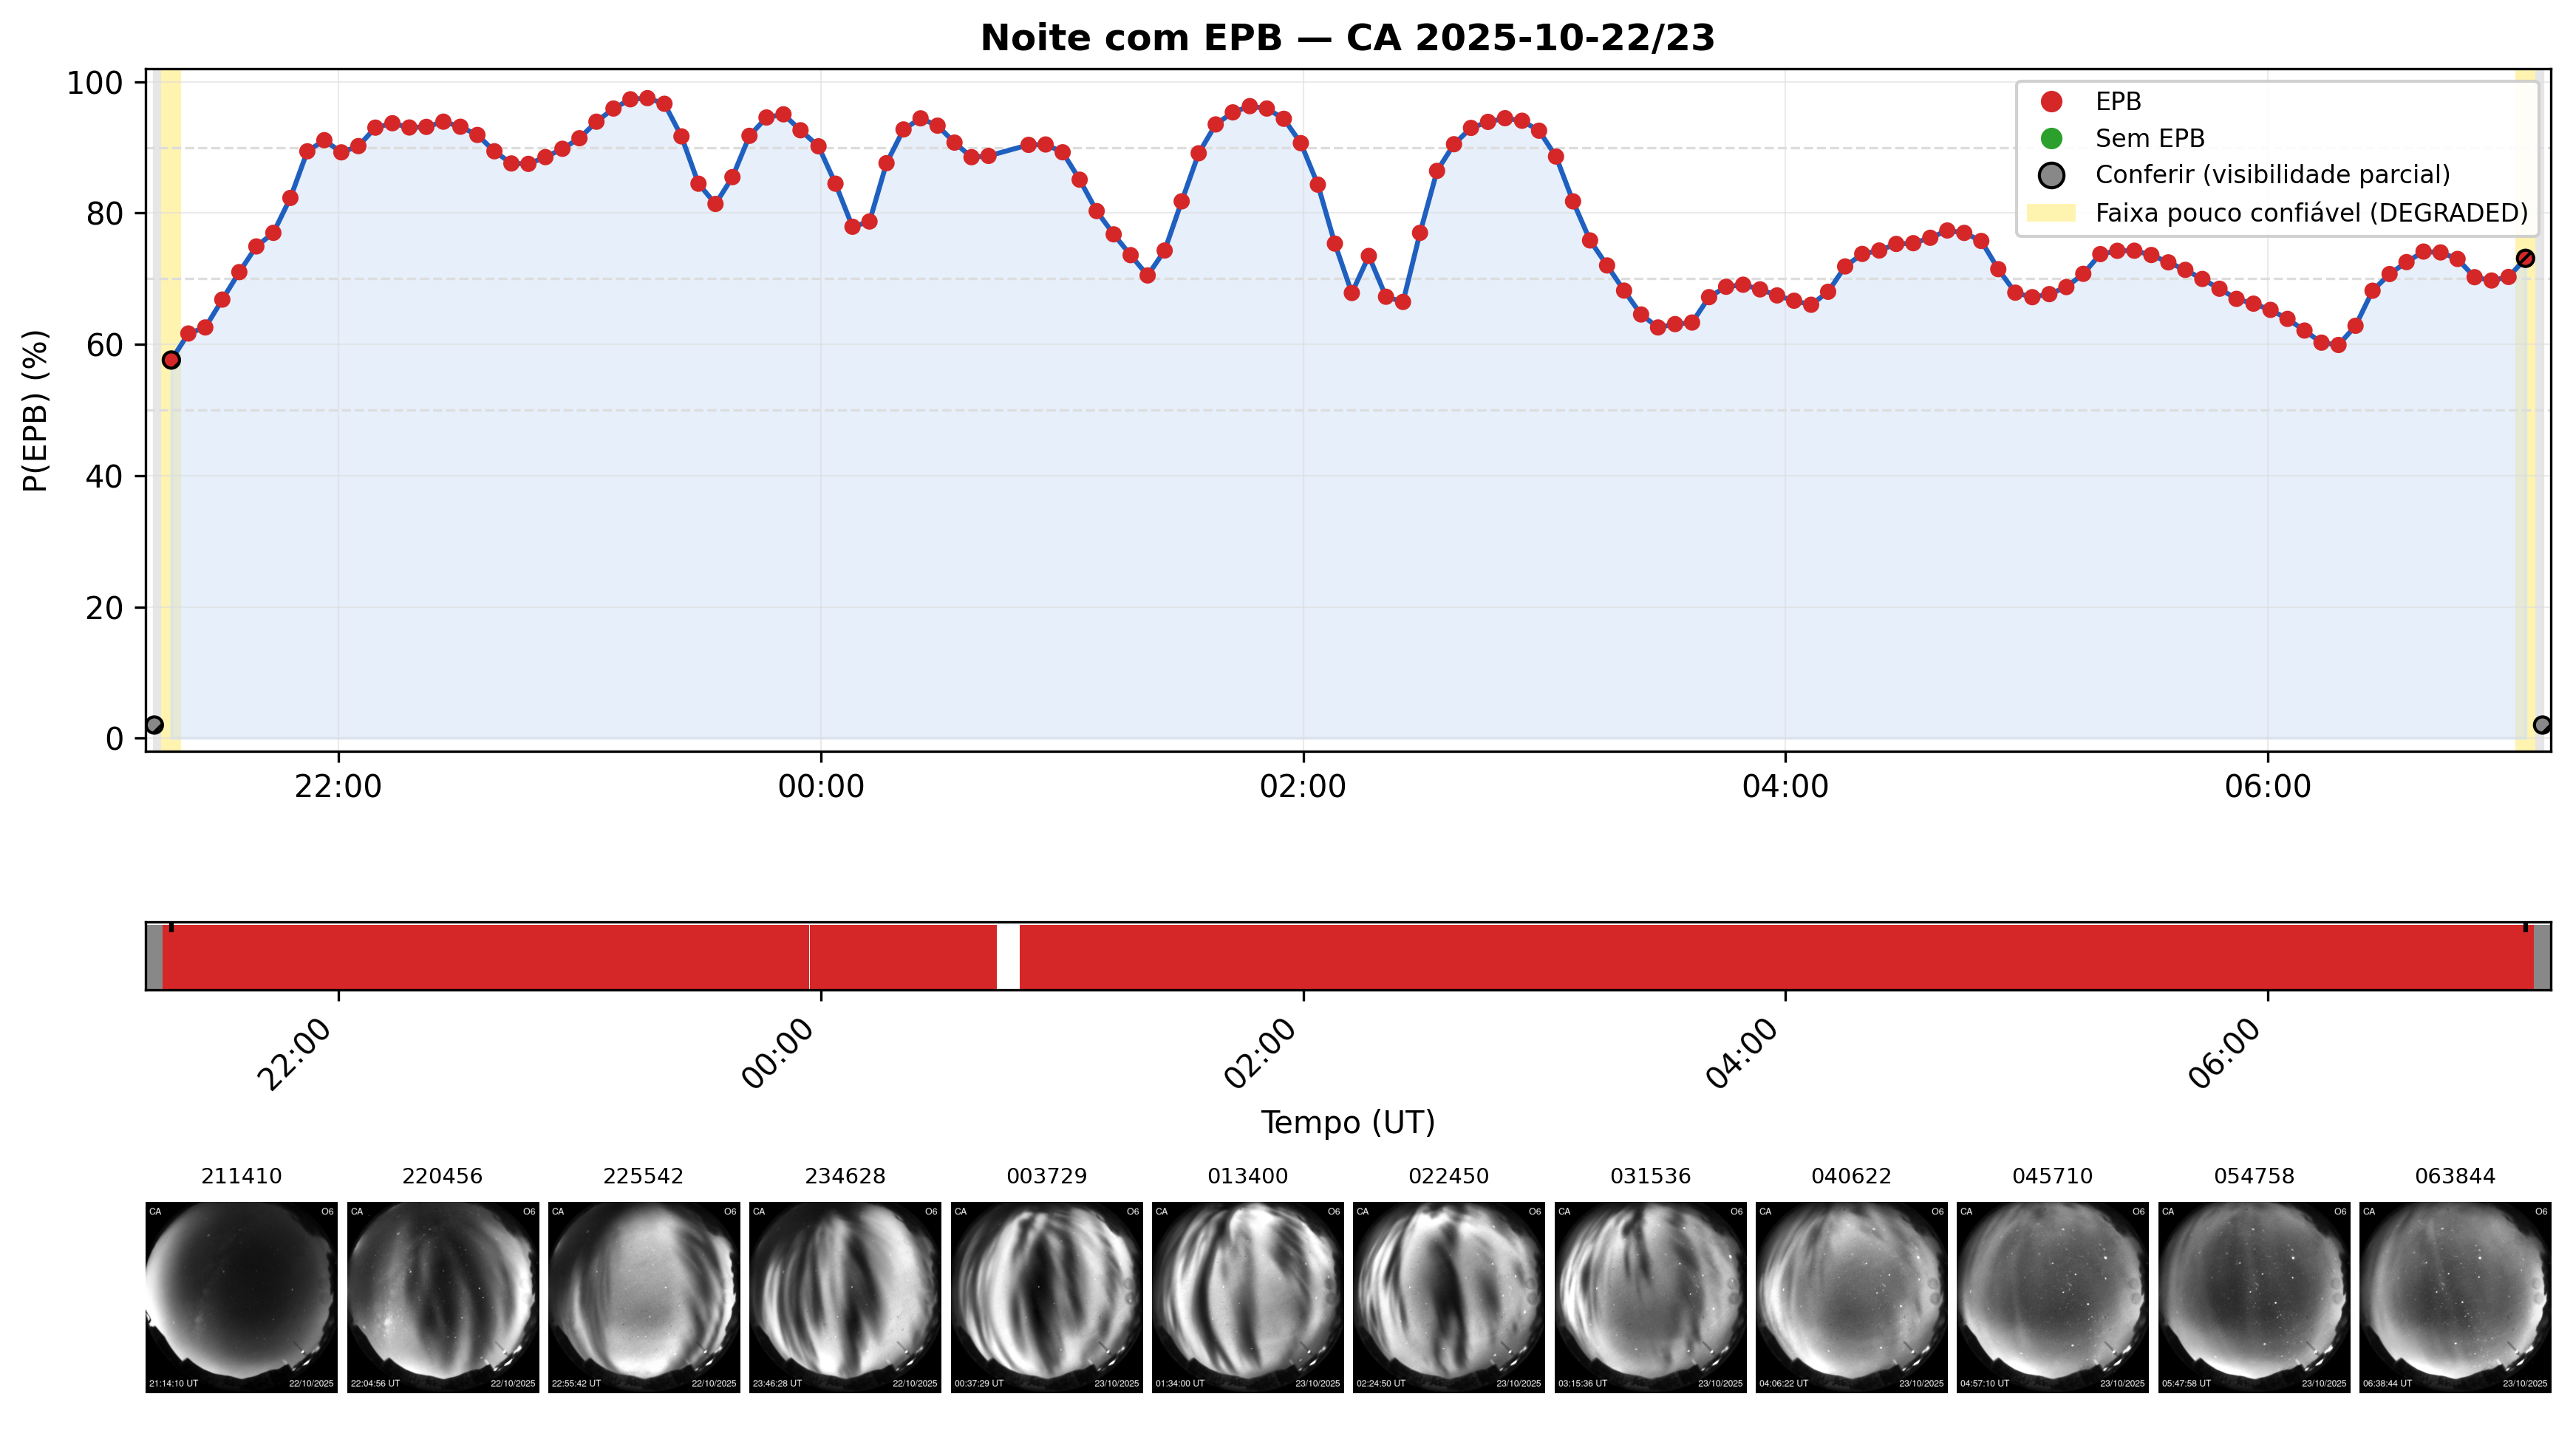
\includegraphics[width=0.98\linewidth,height=6.6cm,keepaspectratio]{figs/temporal_with_epb.png}
        \end{tikzfigure}

        \vspace{0.25em}
        \posteritem{Quiet Sequence (BJL, 230 frames)}{Zero false alarms over 10.5 hours of continuous observation; average probability remains at $2.6\%$.}
        \posteritem{Active Sequence (CA, 140 frames)}{Sharp probability jump across the 0.5 threshold upon bubble emergence, sustaining high-confidence tracking ($91.5\%$) until dawn dissipation.}
    }

    % --------------------------------------------------------------------------
    % SECTION 9: CONCLUSIONS & REFERENCES
    % --------------------------------------------------------------------------
    \block{\textbf{9. Conclusions \& References}}{
        \successitem{Breakthrough Synergy}{Physics-informed preprocessing (Gaussian + CLAHE) combined with 2DPCA ($k=5$) and Stacking Ensemble achieves \textbf{99.80\% F1-Score}, \textbf{100\% Sensitivity}, and \textbf{0\% False Alarms}.}
        \successitem{Real-Time Edge Deployment}{Inference takes \textbf{$<5$ ms per image} on standard CPU hardware, enabling direct deployment at remote automated observatories without costly GPU infrastructure.}
        \successitem{Operational Scalability}{Ready for continuous monitoring across the 11-year solar cycle and scalable to multi-instrument data fusion (GNSS TEC scintillation, Digisondes, and radar).}

        \vspace{0.6em}
        {\color{NavyPrimary}\hrule height 1.5pt}
        \vspace{0.5em}

        {\bfseries\fontsize{15}{18}\selectfont\color{NavyPrimary} Key References \& Acknowledgments:}\par\vspace{4pt}
        {\fontsize{13.5}{17.5}\selectfont
        \noindent\textbf{[1]} J.~Zhong et al., ``Automatic Detection and Feature Extraction of EPBs...'', \textit{Space Weather}, 23, 2025.\par\vspace{3pt}
        \noindent\textbf{[2]} D.~Okoh et al., ``A Bootstrapping CNN Technique for Optimizing Automated Detection...'', \textit{Earth Space Sci.}, 12, 2025.\par\vspace{3pt}
        \noindent\textbf{[3]} L.~Githio et al., ``A Machine Learning Approach for Estimating EPB Drift Velocities...'', \textit{Adv. Space Res.}, 74, 2024.\par\vspace{3pt}
        \noindent\textbf{[4]} M.~Yacoub et al., ``Automatic Detection of EPBs Using 2DPCA and XAI'', \textit{Mach. Learn. Knowl. Extr.}, 7, 2025.\par\vspace{3pt}
        \noindent\textbf{[5]} T.~Thanakulketsarat et al., ``Classification of EPBs Using CNN and SVM'', \textit{Earth Planets Space}, 75, 2023.\par
        }
        
        \vspace{0.6em}
        {\fontsize{12.5}{15.5}\selectfont\color{TextMuted}
        \textbf{Acknowledgments:} The authors thank EMBRACE/INPE for observational data, and acknowledge institutional support from UFPB, UFCG, CAPES, and CNPq.
        \quad $\vert$ \quad \textbf{Contact:} Alberto I. C. Vieira (\texttt{albertoivo@gmail.com})
        }
    }

\end{columns}

\end{document}
